\documentclass{article}
\usepackage{graphicx} % Required for inserting images
\usepackage{hyperref}
\usepackage{tikz}
\usepackage{tabularray}
\usepackage{pgfplots}
\usepackage{float}
\usepackage{listings}
\title{Optimization of Numerical Benchmark Functions Using the Genetic Algorithm}
\author{Denis Crismariu}
\date{\today}



\usepackage{color}

\definecolor{dkgreen}{rgb}{0,0.6,0}
\definecolor{gray}{rgb}{0.5,0.5,0.5}
\definecolor{mauve}{rgb}{0.58,0,0.82}

\lstset{frame=tb,
	language=Python,
	aboveskip=3mm,
	belowskip=3mm,
	showstringspaces=false,
	columns=flexible,
	basicstyle={\small\ttfamily},
	numbers=none,
	numberstyle=\tiny\color{gray},
	keywordstyle=\color{blue},
	commentstyle=\color{dkgreen},
	stringstyle=\color{mauve},
	breaklines=true,
	breakatwhitespace=true,
	tabsize=3,
}



\begin{document}

\maketitle

\abstract

This report investigates the application of Genetic Algorithms (GA) for optimizing mathematical functions, focusing on the implementation and experimentation with different optimization techniques to enhance the performance of the GA. The study compares the results of a newly optimized GA with a previously implemented GA. Through detailed experimentation, we evaluate the efficiency and accuracy of the new GA on four benchmark functions: De Jong’s, Schwefel’s, Rastrigin’s, and Michalewicz’s. This report aims to provide insights into the effectiveness of various optimization strategies and encoding methods in genetic algorithms and suggests potential areas for further research and improvement.Our experiments show that the new Genetic Algorithm has 40\% less error but is 190\% slower compared to the previous version of the Genetic Algorithm.

\section{Introduction}
This report details the use of Genetic Algorithms (GA) for optimizing mathematical functions and compares the results of a newly optimized GA with a previously implemented GA. The study focuses on the implementation and experimentation with different optimization techniques to enhance the performance of the GA. Specifically, our objective is to search for the minima of four benchmark functions: De Jong’s, Schwefel’s, Rastrigin’s, and Michalewicz’s.

The GA starts with an initial population of potential solutions, represented as binary strings. Each generation involves fitness evaluation, selection, crossover, and mutation.

This report aims to provide a detailed analysis of the new GA's performance on the benchmark functions, highlighting the impact of different optimization strategies and encoding methods. By comparing the performance of the new GA with the previously implemented GA, we seek to understand the trade-offs involved and explore potential strategies for enhancing the algorithms' performance. The findings of this study could inform the development of more robust optimization techniques for a wide range of applications. Our experiments show that the new Genetic Algorithm has 40\% less error but is 190\% slower compared to the previous version of the Genetic Algorithm.



\section{Changes and Improvements}

\subsection{Comparison in Pseudocode}
To illustrate the changes and improvements made to the Genetic Algorithm , we present a comparison in pseudocode between the previous implementation and the new optimized version.
\begin{lstlisting}
# Basic Genetic Algorithm
	for e in [1,epoch]:
		evaluation()
		copy_the_best() # copy only top 1
		for x in [1,size): 
			y1 = select()
			y2 = select()
			x = crossover(y1,y2)
			mutate(x)
			
#__________VS__________

# New Genetic Algorithm
	for e in [1,epoch]:
		if g > e/epoch: # switch to graycode for the last g%
			switch_to_graycode()
		evaluation()
		copy_elit(p) # copy top p%
		for x in [p*size,size): 
			y1 = select()
			y2 = select()
			x = crossover(y1,y2)
			mutate(x)
\end{lstlisting}
\subsection{Comparison of Fitness Functions \& Graycode Usage}
\begin{table}[H]
	\centering
	\begin{tblr}{
			colspec={X[0.4,l] X[0.4,l] X[1,l] X[0.3,l]},
			cell{1}{1} = {c=2}{},
			cell{1}{3} = {c},
			cell{1}{4} = {c},
			cell{2}{1} = {r=2}{c},
			cell{4}{1} = {r=2}{c},
			cell{6}{1} = {r=2}{c},
			cell{8}{1} = {r=2}{c},
			vlines,
			hline{1-2,4,6,8,10} = {-}{},
			hline{3,5,7,9} = {2-4}{},
		}
		&          & Fitness function    & Graycode \\
		Rastrigin & Basic AG & $f_2 = \left(\frac{(max - f_1)}{(max - min + \epsilon)} + 1\right)^2$ &  0\%\\
		& New AG & $f_2 = \left(\frac{(max - f_1)}{(max - min + \epsilon)} + 1\right)^{0.5}$    & 50\%   \\
		Michalewics & Basic AG & $f_2 = \left(\frac{(max - f_1)}{(max - min + \epsilon)} + 1\right)^3$ &  0\%\\
		& New AG & $f_2 = \left(\frac{(max - f_1)}{(max - min + \epsilon)} + 1\right)^3$   & 50\%   \\
		De Jong & Basic AG & $f_2=\frac{1}{f_1+\epsilon}$ &  0\%\\
		& New AG & $f_2=\frac{1}{f_1+\epsilon}$   & 50\%   \\
		Schwefel & Basic AG & $f_2 = \left(\frac{(max - f_1)}{(max - min + \epsilon)} + 1\right)^2$  &  0\%\\
		& New AG & $f_2 = \left(\frac{(max - f_1)}{(max - min + \epsilon)} + 1\right)^{0.8}$    & 0\%   
	\end{tblr}
	
\end{table}


\section{Methods \& Implementation}

The implementation of the upgraded Genetic Algorithm (GA) involves setting parameters that influence its efficiency. We set the population size to 100, the mutation probability to $\frac{1}{L}$, and 2000 generations. Additionally, we set the precision to be $10^{-5}$ and the dimensions to 5, 10, and 30.

Our approach to the GA follows a distinct order: fitness evaluation, selection, crossover, and mutation.

Each generation concludes with the fitness evaluation of the new population. The fitness of each individual is calculated based on the objective function we aim to minimize. We experimented with different fitness evaluation functions to enhance the performance of the genetic algorithm.

The selection and crossover process takes place next. In this phase, two parents are selected based on a binary search on cumulative fitness for faster selection. Each chromosome from the parents has a 50\% chance of being passed to the offspring, creating two new offspring that inherit a blend of genetic material from both parents. Additionally, the top p\% of individuals from the current generation are copied directly to the next generation to ensure that the highest fitness solutions are preserved.

The mutation step, applied to the newly created individuals with the best from the last generation as an exception, introduces random changes in the genetic makeup of the individuals. This process, governed by the optimized mutation probability, is vital for injecting new genetic traits into the population, thereby enhancing its diversity and aiding in the exploration of new areas in the solution space. This is done by flipping the bits in the binary strings at a probability set in the initial phase.

A significant change in the new GA is the conversion to graycode representation for the last portion of the generations. This switch helps in reducing the error by providing a more efficient encoding method. The new GA also runs for twice the number of generations compared to the unupgraded version, allowing more time for the algorithm to converge to a better solution.

These changes collectively contribute to the enhanced performance of the new Genetic Algorithm, making it more accurate but also more computationally intensive.



\section{Experimental results}
The 4 benchmarked functions are the following:

\subsection{Rastrigin Function\cite{Rastrigin}}

$$ f(x) = A \cdot n + \sum_{i=1}^n \left[ x_i^2 - A \cdot cos(2 \pi x_i) \right],
A = 10, x_i \in \left[ -5.12, 5.15 \right]$$

The global minima is located at $f(x)=0; x(i)=0,  \forall i=1:n $
\begin{figure}[!h]
  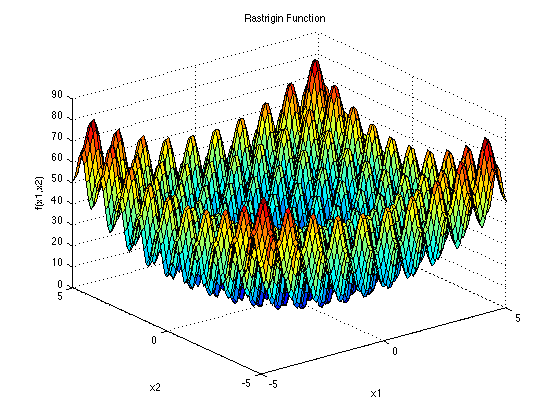
\includegraphics[width=\textwidth,height=\textheight,keepaspectratio]{rastr.png}
  \caption{Rastrigin Function\cite{rast_img}}
\end{figure}
\begin{table}[H]
\caption{Values based on 30 runs}
\begin{tblr}{
colspec={X[0.96,l] X[1.7,l] X[1,l] X[1,l] X[1,l] X[1,l]},
rowsep=0.01pt,  % Reduce the vertical padding between cell contents and borders
  cell{1}{1} = {c=2}{},
  cell{2}{1} = {r=4}{c},
  cell{6}{1} = {r=4}{c},
  cell{10}{1} = {r=4}{c},
  vlines,
  hline{1-2,6,10,14} = {-}{},
  hline{3-5,7-9,11-13} = {2-7}{},
}
     &               & GA & GA opt\\
D = 5 & Mean error   & 0.001 & 0.000\\
      &   SDev error & 0.005 & 0.000\\
      &   Min error  & 0.000 & 0.000\\
      &   Max error  & 0.031 & 0.000\\

D = 10 & Mean error & 3.935 & 0.000\\
     &   SDev error & 2.148 & 0.000\\
     &   Min error  & 1.040 & 0.000\\
     &   Max error  & 9.419 & 0.000\\

D = 30 & Mean error & 31.982 & 6.973\\
     &   SDev error & 6.757 & 3.993\\
     &   Min error  & 19.837 & 2.069\\
     &   Max error  & 46.042 & 15.921\\
\end{tblr}
\caption{Hill Climbing time (in seconds) based on 30 runs}
\begin{tblr}{
colspec={X[0.96,l] X[1.7,l] X[1,l] X[1,l] X[1,l] X[1,l]},
rowsep=0.01pt,  % Reduce the vertical padding between cell contents and borders
  cell{1}{1} = {c=2}{},
  cell{2}{1} = {r=4}{c},
  cell{6}{1} = {r=4}{c},
  cell{10}{1} = {r=4}{c},
  vlines,
  hline{1-2,6,10,14} = {-}{},
  hline{3-5,7-9,11-13} = {2-7}{},
}
     &              & GA & GA opt\\
D = 5 & Mean time  & 0.207 & 0.424\\
     &   SDev time & 0.005 & 0.006\\
     &   Min time  & 0.205 & 0.420\\
     &   Max time  & 0.234 & 0.452\\

D = 10 & Mean time & 0.354 & 0.752\\
     &   SDev time & 0.005 & 0.017\\
     &   Min time  & 0.351 & 0.741\\
     &   Max time  & 0.366 & 0.825\\

D = 30 & Mean time & 1.014 & 2.143\\
     &   SDev time & 0.026 & 0.026\\
     &   Min time  & 0.967 & 2.128\\
     &   Max time  & 1.043 & 2.250\\
\end{tblr}
\end{table}
\newpage
\subsection{Michalewicz Function\cite{michal}}

$$
f(x) = - \sum_{i=1}^n \sin \left(x_i \right)\sin^{2m}\left(\frac{ix_i^2}{\pi}\right),
x_i \in \left[ 0 , \pi \right]$$

The global minima is located at $n=5: f (x) = -4.687$, for $n=10: f (x) = -9.660$ and for  $n=30: f (x) = -29.630$\cite{glob_min}.

\begin{figure}[!h]
  \centering
  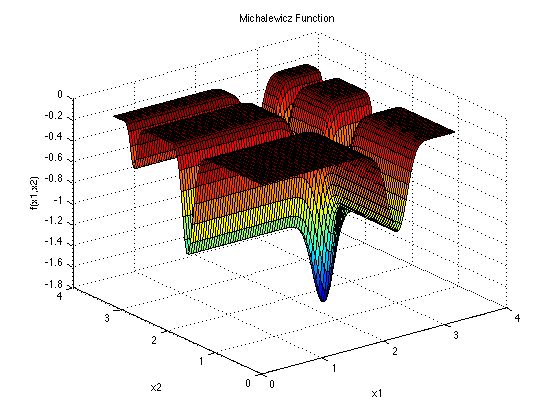
\includegraphics[width=\textwidth,height=\textheight,keepaspectratio]{michal.png}
  \caption{Michalewicz Function\cite{michal_img}}
\end{figure}


\begin{table}[H]
\caption{Values based on 30 runs}
\begin{tblr}{
colspec={X[0.96,l] X[1.7,l] X[1,l] X[1,l] X[1,l] X[1,l]},
rowsep=0.01pt,  % Reduce the vertical padding between cell contents and borders
  cell{1}{1} = {c=2}{},
  cell{2}{1} = {r=4}{c},
  cell{6}{1} = {r=4}{c},
  cell{10}{1} = {r=4}{c},
  vlines,
  hline{1-2,6,10,14} = {-}{},
  hline{3-5,7-9,11-13} = {2-7}{},
}
     &              & GA & GA opt\\
D = 5 & Mean error  & 0.007 & 0.000\\
     &   SDev error & 0.086 & 0.057\\
     &   Min error  & 0.000 & 0.000\\
     &   Max error  & 0.331 & 0.150\\

D = 10 & Mean error & 0.325 & 0.296\\
     &   SDev error & 0.213 & 0.193\\
     &   Min error  & 0.016 & 0.000\\
     &   Max error  & 0.884 & 0.770\\

D = 30 & Mean error & 3.675 & 2.116\\
     &   SDev error & 0.692 & 0.511\\
     &   Min error  & 2.864 & 1.175\\
     &   Max error  & 5.559 & 3.351\\
\end{tblr}
\caption{Hill Climbing time (in seconds) based on 30 runs}
\begin{tblr}{
colspec={X[0.96,l] X[1.7,l] X[1,l] X[1,l] X[1,l] X[1,l]},
rowsep=0.01pt,  % Reduce the vertical padding between cell contents and borders
  cell{1}{1} = {c=2}{},
  cell{2}{1} = {r=4}{c},
  cell{6}{1} = {r=4}{c},
  cell{10}{1} = {r=4}{c},
  vlines,
  hline{1-2,6,10,14} = {-}{},
  hline{3-5,7-9,11-13} = {2-7}{},
}
     &              & GA & GA opt\\
D = 5 & Mean time  & 0.203 & 0.395\\
     &   SDev time & 0.002 & 0.002\\
     &   Min time  & 0.196 & 0.394\\
     &   Max time  & 0.211 & 0.403\\

D = 10 & Mean time & 0.384 & 0.738\\
     &   SDev time & 0.004 & 0.002\\
     &   Min time  & 0.367 & 0.735\\
     &   Max time  & 0.399 & 0.743\\

D = 30 & Mean time & 1.067 & 2.013\\
     &   SDev time & 0.010 & 0.010\\
     &   Min time  & 1.035 & 1.993\\
     &   Max time  & 1.098 & 2.039\\

\end{tblr}
\end{table}
\newpage
\subsection{De Jong Function\cite{dejong}}

$$
f(x) = \sum^n_{i=1}{x_i^2},
x_i \in \left[ -5.12 , 5.12 \right]
$$

The global minima is located at $f(x)=0; x(i)=0,  \forall i=1:n $

\begin{figure}[!h]
  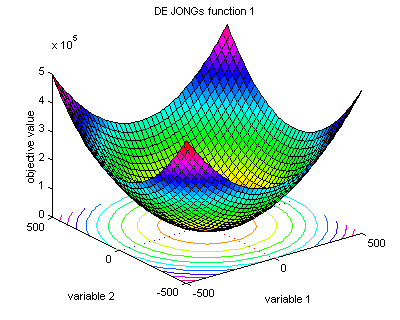
\includegraphics[width=\textwidth,height=\textheight,keepaspectratio]{dejong.png}
  \caption{De Jong Function Function\cite{dejong_img}}
\end{figure}

\begin{table}[H]
\caption{Values based on 30 runs}
\begin{tblr}{
colspec={X[0.96,l] X[1.7,l] X[1,l] X[1,l] X[1,l] X[1,l]},
rowsep=0.01pt,  % Reduce the vertical padding between cell contents and borders
  cell{1}{1} = {c=2}{},
  cell{2}{1} = {r=4}{c},
  cell{6}{1} = {r=4}{c},
  cell{10}{1} = {r=4}{c},
  vlines,
  hline{1-2,6,10,14} = {-}{},
  hline{3-5,7-9,11-13} = {2-7}{},
}
     &              & GA & GA opt\\
D = 5 & Mean error  & 0.000 & 0.000\\
     &   SDev error & 0.000 & 0.000\\
     &   Min error  & 0.000 & 0.000\\
     &   Max error  & 0.000 & 0.000\\

D = 10 & Mean error & 0.000 & 0.000\\
     &   SDev error & 0.000 & 0.000\\
     &   Min error  & 0.000 & 0.000\\
     &   Max error  & 0.000 & 0.000\\

D = 30 & Mean error & 0.000 & 0.000\\
     &   SDev error & 0.000 & 0.000\\
     &   Min error  & 0.000 & 0.000\\
     &   Max error  & 0.000 & 0.000\\
       
\end{tblr}
\caption{Hill Climbing time (in seconds) based on 30 runs}
\begin{tblr}{
colspec={X[0.96,l] X[1.7,l] X[1,l] X[1,l] X[1,l] X[1,l]},
rowsep=0.01pt,  % Reduce the vertical padding between cell contents and borders
  cell{1}{1} = {c=2}{},
  cell{2}{1} = {r=4}{c},
  cell{6}{1} = {r=4}{c},
  cell{10}{1} = {r=4}{c},
  vlines,
  hline{1-2,6,10,14} = {-}{},
  hline{3-5,7-9,11-13} = {2-7}{},
}
     &              & GA & GA opt\\
D = 5 & Mean time  & 0.192 & 0.377\\
     &   SDev time & 0.001 & 0.003\\
     &   Min time  & 0.192 & 0.376\\
     &   Max time  & 0.198 & 0.388\\

D = 10 & Mean time & 0.337 & 0.659\\
     &   SDev time & 0.005 & 0.011\\
     &   Min time  & 0.336 & 0.653\\
     &   Max time  & 0.369 & 0.712\\

D = 30 & Mean time & 0.961 & 1.875\\
     &   SDev time & 0.007 & 0.021\\
     &   Min time  & 0.941 & 1.850\\
     &   Max time  & 0.973 & 1.935\\
\end{tblr}
\end{table}
\newpage
\subsection{Schwefel Function\cite{schwef}}

$$
f(x) = 418.982n - \sum_{i=1}^n{x_i\sin(\sqrt{\left|x_i\right|})},
x_i \in \left[ -500 , 500 \right]
$$

The global minima is located at $f(x)=0; x(i)=0,  \forall i=1:n $

\begin{figure}[!h]
  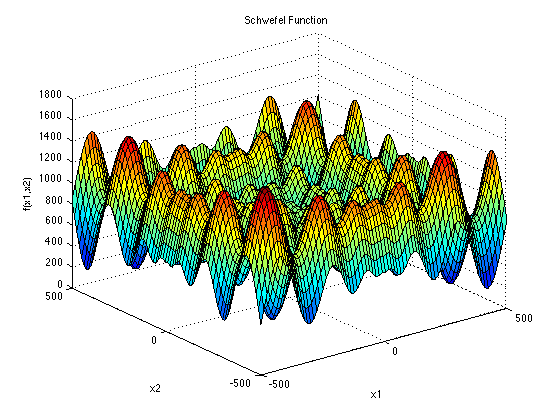
\includegraphics[width=\textwidth,height=\textheight,keepaspectratio]{schwef.png}
  \caption{Schwefel Function\cite{schwef_img}}
\end{figure}

\begin{table}[H]
\caption{Values based on 30 runs}
\begin{tblr}{
colspec={X[0.96,l] X[1.7,l] X[1,l] X[1,l] X[1,l] X[1,l]},
rowsep=0.01pt,  % Reduce the vertical padding between cell contents and borders
  cell{1}{1} = {c=2}{},
  cell{2}{1} = {r=4}{c},
  cell{6}{1} = {r=4}{c},
  cell{10}{1} = {r=4}{c},
  vlines,
  hline{1-2,6,10,14} = {-}{},
  hline{3-5,7-9,11-13} = {2-7}{},
}
     &              & GA & GA opt\\
D = 5 & Mean error  & 0.177 & 0.208\\
     &   SDev error & 0.131 & 0.126\\
     &   Min error  & 0.002 & 0.000\\
     &   Max error  & 0.439 & 0.518\\

D = 10 & Mean error & 30.249 & 0.417\\
     &   SDev error & 59.370 & 0.161\\
     &   Min error  & 0.486 & 0.311 \\
     &   Max error  & 273.941 & 0.830\\

D = 30 & Mean error & 845.000 & 336.127\\
     &   SDev error & 291.677 & 181.053\\
     &   Min error  & 455.446 & 104.295\\
     &   Max error  & 1952.879 & 891.062\\
\end{tblr}
\caption{Hill Climbing time (in seconds) based on 30 runs}
\begin{tblr}{
colspec={X[0.96,l] X[1.7,l] X[1,l] X[1,l] X[1,l] X[1,l]},
rowsep=0.01pt,  % Reduce the vertical padding between cell contents and borders
  cell{1}{1} = {c=2}{},
  cell{2}{1} = {r=4}{c},
  cell{6}{1} = {r=4}{c},
  cell{10}{1} = {r=4}{c},
  vlines,
  hline{1-2,6,10,14} = {-}{},
  hline{3-5,7-9,11-13} = {2-7}{},
}
     &              & GA & GA opt\\
D = 5 & Mean time  & 0.260 & 0.430\\
     &   SDev time & 0.011 & 0.001\\
     &   Min time  & 0.249 & 0.429\\
     &   Max time  & 0.299 & 0.433\\

D = 10 & Mean time & 0.476 & 0.809\\
     &   SDev time & 0.017 & 0.006\\
     &   Min time  & 0.460 & 0.808\\
     &   Max time  & 0.524 & 0.842\\

D = 30 & Mean time & 1.353 & 2.296\\
     &   SDev time & 0.052 & 0.022\\
     &   Min time  & 1.303 & 2.285\\
     &   Max time  & 1.511 & 2.381\\
\end{tblr}
\end{table}

\section{Comparing Methods}
Comparing the upgraded Genetic Algorithm (GA) to the unupgraded version, we observed that the new GA achieves significantly better accuracy but at the cost of increased computational time. Specifically, our experiments show that the upgraded GA has 40\% less error but is 190\% slower compared to the unupgraded GA. This improvement in accuracy is primarily due to the conversion to graycode and the doubling of the number of generations.

\section{Conclusions}
In conclusion, the upgraded Genetic Algorithm (GA) demonstrates a significant improvement in accuracy, achieving 40\% less error compared to the unupgraded version. However, this enhancement comes at the cost of increased computational time, with the new GA being 190\% slower. The primary factors contributing to this improvement are the conversion to graycode representation for the last portion of the generations and the doubling of the number of generations. These changes allow the algorithm to explore the solution space more effectively and converge to better solutions, albeit with a higher computational cost. This trade-off between accuracy and speed highlights the importance of selecting the appropriate optimization strategy based on the specific requirements and constraints of the application.


\begin{thebibliography}{9}

\bibitem{rast_img}
Authors: Sonja Surjanovic \& Derek Bingham, Simon Fraser University \\ Rastrigin's Function rendered image.
  \url{https://www.sfu.ca/~ssurjano/rastr.html}

\bibitem{Rastrigin}
  Rastrigin, L. A. "Systems of extremal control." Mir, Moscow (1974).

\bibitem{michal_img}
Authors: Sonja Surjanovic \& Derek Bingham, Simon Fraser University \\ Michalewicz's Function rendered image.
  \url{https://www.sfu.ca/~ssurjano/michal.html}

\bibitem{michal}
    Michalewicz, Zbigniew. "A survey of constraint handling techniques in evolutionary computation methods." (1995).

\bibitem{dejong_img}
Dejong's Function rendered image.
  \url{http://www.geatbx.com/docu/fcnindex-msh_f1_500-2.gif}

\bibitem{dejong}
De Jong, Kenneth Alan. An analysis of the behavior of a class of genetic adaptive systems. University of Michigan, 1975.

\bibitem{schwef_img}
Authors: Sonja Surjanovic \& Derek Bingham, Simon Fraser University \\ Schwefel's Function rendered image.
  \url{https://www.sfu.ca/~ssurjano/schwef.html}

\bibitem{schwef}
Bäck, Thomas, and Hans-Paul Schwefel. "An overview of evolutionary algorithms for parameter optimization." Evolutionary computation 1.1 (1993): 1-23.

\bibitem{glob_min}
Vanaret, Charlie, et al. "Certified global minima for a benchmark of difficult optimization problems." arXiv preprint arXiv:2003.09867(2020).


\end{thebibliography} 


\end{document}




